% ============================================================
%  SYSTEM BLOCK DIAGRAM — strict column layout, no diagonal arrows
% ============================================================
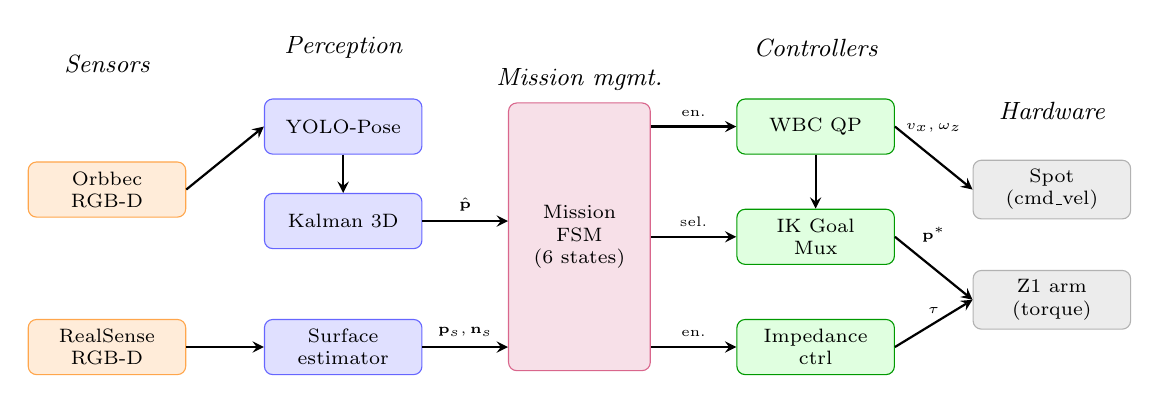
\begin{tikzpicture}[
    >=stealth,
    arr/.style    = {->, thick},
    box/.style    = {rectangle, draw, rounded corners=3pt,
                     minimum width=2.0cm, minimum height=0.70cm,
                     font=\scriptsize, align=center, fill=white},
    sensor/.style = {box, fill=orange!15, draw=orange!70},
    percep/.style = {box, fill=blue!12,   draw=blue!60},
    fsmbox/.style = {box, fill=purple!12, draw=purple!60,
                     minimum width=1.8cm, minimum height=3.4cm},
    ctrl/.style   = {box, fill=green!12,  draw=green!60!black},
    hw/.style     = {box, fill=gray!15,   draw=gray!60},
    lbl/.style    = {font=\small\itshape},
  ]

  % ── Column x: 0  3.0  6.0  9.0  12.0 ───────────────────────
  % ── Row y:  top=1.4  mid=0  bot=-1.4 ────────────────────────

  % SENSORS
  \node[sensor] (orb)  at ( 0.0,  1.0) {Orbbec\\RGB-D};
  \node[sensor] (rs)   at ( 0.0, -1.0) {RealSense\\RGB-D};

  % PERCEPTION
  \node[percep] (yolo) at ( 3.0,  1.8) {YOLO-Pose};
  \node[percep] (kf)   at ( 3.0,  0.6) {Kalman 3D};
  \node[percep] (surf) at ( 3.0, -1.0) {Surface\\estimator};

  % FSM
  \node[fsmbox] (fsm)  at ( 6.0,  0.4) {Mission\\FSM\\(6 states)};

  % CONTROLLERS
  \node[ctrl] (wbc)  at ( 9.0,  1.8) {WBC QP};
  \node[ctrl] (mux)  at ( 9.0,  0.4) {IK Goal\\Mux};
  \node[ctrl] (imp)  at ( 9.0, -1.0) {Impedance\\ctrl};

  % HARDWARE
  \node[hw] (spot) at (12.0,  1.0) {Spot\\(cmd\_vel)};
  \node[hw] (z1)   at (12.0, -0.4) {Z1 arm\\(torque)};

  % ── Sensors → Perception ────────────────────────────────────
  \draw[arr] (orb.east)  -- (yolo.west);
  \draw[arr] (yolo.south) -- (kf.north);
  \draw[arr] (rs.east)   -- (surf.west);

  % ── Perception → FSM ────────────────────────────────────────
  \draw[arr] (kf.east)   -- node[above,font=\tiny]{$\hat{\mathbf{p}}$}
             (fsm.west |- kf);
  \draw[arr] (surf.east) -- node[above,font=\tiny]{$\mathbf{p}_s,\mathbf{n}_s$}
             (fsm.west |- surf);

  % ── FSM → Controllers ───────────────────────────────────────
  \draw[arr] (fsm.east |- wbc) -- node[above,font=\tiny]{en.} (wbc.west);
  \draw[arr] (fsm.east |- mux) -- node[above,font=\tiny]{sel.}(mux.west);
  \draw[arr] (fsm.east |- imp) -- node[above,font=\tiny]{en.} (imp.west);

  % ── WBC → Mux ───────────────────────────────────────────────
  \draw[arr] (wbc.south) -- (mux.north);

  % ── WBC → Spot (separate, horizontal) ───────────────────────
  \draw[arr] (wbc.east) --
           node[above,font=\tiny,yshift=2mm]{$v_x,\omega_z$} (spot.west);

  % ── Mux → Z1 ────────────────────────────────────────────────
  \draw[arr] (mux.east) --
             node[above,font=\tiny,yshift=2mm]{$\mathbf{p}^*$}
             (z1.west);

  % ── Imp → Z1 ────────────────────────────────────────────────
  \draw[arr] (imp.east) --
             node[above,font=\tiny]{$\boldsymbol{\tau}$}
             (z1.west);

  % ── Column labels ────────────────────────────────────────────
  \node[lbl] at ( 0.0,  2.6) {Sensors};
  \node[lbl] at ( 3.0,  2.8) {Perception};
  \node[lbl] at ( 6.0,  2.4) {Mission mgmt.};
  \node[lbl] at ( 9.0,  2.8) {Controllers};
  \node[lbl] at (12.0,  2.0) {Hardware};

\end{tikzpicture}
